% !TEX TS-program = pdflatex
% !TEX encoding = UTF-8 Unicode

% This file is a template using the "beamer" package to create slides for a talk or presentation
% - Talk at a conference/colloquium.
% - Talk length is about 20min.
% - Style is ornate.

% MODIFIED by Jonathan Kew, 2008-07-06
% The header comments and encoding in this file were modified for inclusion with TeXworks.
% The content is otherwise unchanged from the original distributed with the beamer package.

\documentclass{beamer}
%\usepackage[demo]{graphicx}
%\usepackage{caption}
\usepackage{subcaption}
\captionsetup{compatibility=false}
\usepackage[export]{adjustbox}
\usepackage{algorithm,algpseudocode}
% Copyright 2004 by Till Tantau <tantau@users.sourceforge.net>.
%
% In principle, this file can be redistributed and/or modified under
% the terms of the GNU Public License, version 2.
%
% However, this file is supposed to be a template to be modified
% for your own needs. For this reason, if you use this file as a
% template and not specifically distribute it as part of a another
% package/program, I grant the extra permission to freely copy and
% modify this file as you see fit and even to delete this copyright
% notice. 


\mode<presentation>
{
  \usetheme{Warsaw}
  % or ...

  \setbeamercovered{transparent}
  % or whatever (possibly just delete it)
}


\usepackage[english]{babel}
% or whatever

\usepackage[utf8]{inputenc}
% or whatever

\usepackage{times}
\usepackage[T1]{fontenc}
% Or whatever. Note that the encoding and the font should match. If T1
% does not look nice, try deleting the line with the fontenc.


\title[Parallel Convex Hull] % (optional, use only with long paper titles)
{Parallel Convex Hull}

\subtitle
{Section 5.4 in the book}

\author{Brendan Benshoof} % (optional, use only with lots of authors)
%{Brendan~Benshoof}
% - Give the names in the same order as the appear in the paper.
% - Use the \inst{?} command only if the authors have different
%   affiliation.


\date % (optional, should be abbreviation of conference name)
{Feb 11, 2015}
% - Either use conference name or its abbreviation.
% - Not really informative to the audience, more for people (including
%   yourself) who are reading the slides online

\subject{Theoretical Computer Science}
% This is only inserted into the PDF information catalog. Can be left
% out. 



% If you have a file called "university-logo-filename.xxx", where xxx
% is a graphic format that can be processed by latex or pdflatex,
% resp., then you can add a logo as follows:

% \pgfdeclareimage[height=0.5cm]{university-logo}{university-logo-filename}
% \logo{\pgfuseimage{university-logo}}



% Delete this, if you do not want the table of contents to pop up at
% the beginning of each subsection:
\AtBeginSubsection[]
{
  \begin{frame}<beamer>{Outline}
    \tableofcontents[currentsection,currentsubsection]
  \end{frame}
}


% If you wish to uncover everything in a step-wise fashion, uncomment
% the following command: 

%\beamerdefaultoverlayspecification{<+->}


\begin{document}

\begin{frame}
  \titlepage
\end{frame}

\begin{frame}{Outline}
  \tableofcontents
  % You might wish to add the option [pausesections]
\end{frame}


% Structuring a talk is a difficult task and the following structure
% may not be suitable. Here are some rules that apply for this
% solution: 

% - Exactly two or three sections (other than the summary).
% - At *most* three subsections per section.
% - Talk about 30s to 2min per frame. So there should be between about
%   15 and 30 frames, all told.

% - A conference audience is likely to know very little of what you
%   are going to talk about. So *simplify*!
% - In a 20min talk, getting the main ideas across is hard
%   enough. Leave out details, even if it means being less precise than
%   you think necessary.
% - If you omit details that are vital to the proof/implementation,
%   just say so once. Everybody will be happy with that.

\section{What is a Convex Hull?}

\begin{frame}{What is A Convex Polytope?}
  % - A title should summarize the slide in an understandable fashion
  %   for anyone how does not follow everything on the slide itself.
  \begin{itemize}
  \item
    A polytope is the generalization of a polygon into any number of dimensions.
  \item
    A convex polytope is formed by a Convex-set of points
  \item
    A convex set of points is defined as a set of points such that for every pair of points, the line between those points falls wholly within the set.
  \end{itemize}
  
\end{frame}

\begin{frame}{Examples!}
\begin{figure}
\centering
\begin{subfigure}{.5\textwidth}
  \centering
  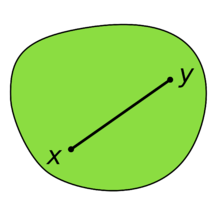
\includegraphics[width=.4\linewidth]{imgs/convex.png}
  \caption{A convex set}
  \label{fig:sub1}
\end{subfigure}%
\begin{subfigure}{.5\textwidth}
  \centering
  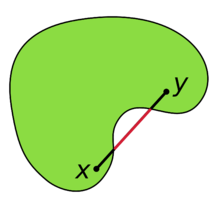
\includegraphics[width=.4\linewidth]{imgs/notconvex.png}
  \caption{A non-convex set}
  \label{fig:sub2}
\end{subfigure}

\label{fig:test}
\end{figure}

\footnote{By Oleg Alexandrov [Public domain], via Wikimedia Commons}
\end{frame}


\begin{frame}{this is a Convex Hull}
  % - A title should summarize the slide in an understandable fashion
  %   for anyone how does not follow everything on the slide itself.
  \begin{itemize}
  \item
    A convex hull is a sub-set of points that describe a hull that contains a convex set and all the points as part of that set.
  \item
  	A convex Hull is often compared to stretching a rubber band around a set of points.
  \item
   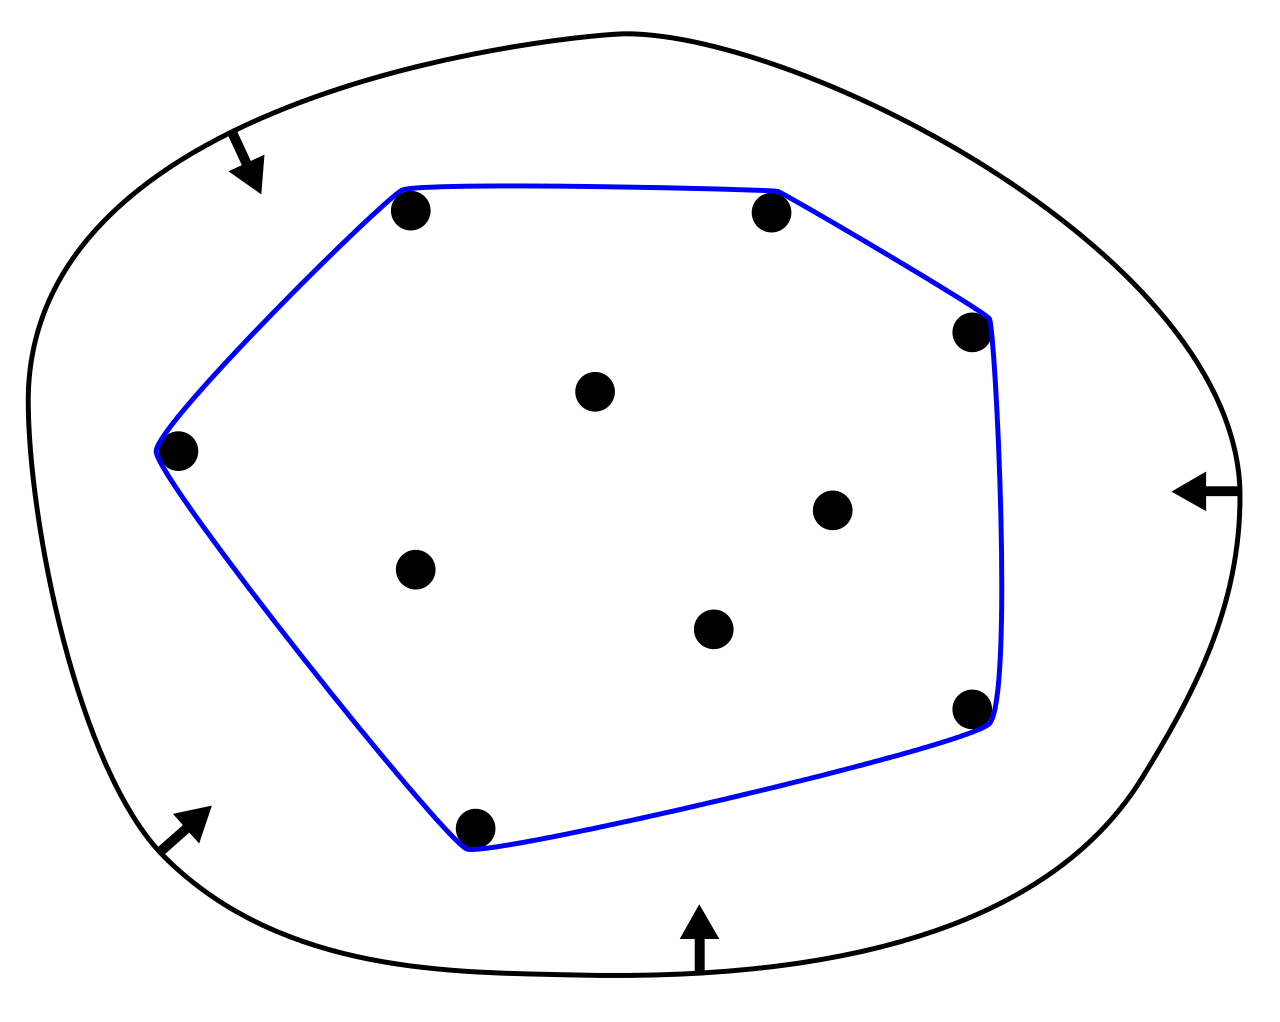
\includegraphics[width=.6\linewidth]{imgs/convex_hull.png}
By Maksim (original); en:User:Pbroks3 (redraw) [Public domain], via Wikimedia Commons
%  \caption{A non-convex set}
  \end{itemize}
  
\end{frame}

\section{Centralized 2d Algorithims}

\begin{frame}{Graham Scan}
\begin{itemize}
\item
	The lowest y point is selected to begin.
\item
	All points are sorted by their angle relative to the horizontal axis at the starting point and pushed into a stack such that the smallest angle is on the top (called the potential point stack).
\item
	starting with the lowest angle the point popped and is pushed onto a stack (the convex hull stack)
\item
	iteratively each angle is popped from the potential stack and pushed to the hull stack.
\item 
	As each item is pushed the angle formed by the last 3 points is calculated
\item
	if the angle is a ``right-turn'' the top item of the hull stack is popped and pushed onto the potential stack and the next item on the hull stack is popped and discarded.
\end{itemize}

\end{frame}




\begin{frame}{Graham Scan Picture}
\begin{figure}
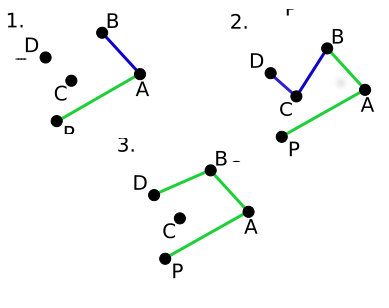
\includegraphics[width=.2\linewidth,center]{imgs/Graham_Scan.png}
    \caption{By User A1 at en.wikipedia (Transferred from en.wikipedia by SreeBot) [GFDL (http://www.gnu.org/copyleft/fdl.html) or CC-BY-SA-3.0 (http://creativecommons.org/licenses/by-sa/3.0/)], via Wikimedia Commons}
\end{figure}

\end{frame}

\begin{frame}{Graham Scan's Properties}

\begin{itemize}
\item
	Time is $O(nlg(n))$ and is dominated by sorting points by angle
\item
	Space is O(n)
\item
	Not efficiently parallelizable. (we could parallelize the sorting step, but not the $O(n)$ ``wrapping'' step.)

\end{itemize}
\end{frame}




%\begin{frame}[]
%\end{frame}

\section{Parallel Algorithms for Convex Hull}

\begin{frame}{Initial Consideration}

\begin{itemize}
\item
	Given $O(n^4)$ processors, we can compute a convex hull of n points in 2d in O(1) time
\item
	assign an array of booleans in shared memory such that each point is assigned a value. Default these values to true.
\item
	for each triplet of points $p_x$, $p_y$, $p_z$ do in parallel: ($n^3$ processors)
	\begin{itemize}
		\item
			for each point p do in parallel:
		\begin{itemize}
			\item
				If p falls inside the triangle $p_x$, $p_y$, $p_z$, mark p False in shared memory
		\end{itemize}	
	\end{itemize}	
	
\item
	The remaining points are the convex hull. (sadly you still need to sort them if you want their order)
\item
	The cost of this algorithm is $O(n^{d+2})$ and we can do better!

\end{itemize}
\end{frame}

\begin{frame}{Divide and Conquer}
Basic Steps of CH(S):
\begin{itemize}
\item
	Split the point set vertically. Solve each half recursively
\item
	If there are 3 or less points in the problem, they form a convex for free
\item
	Merge the results
\end{itemize}
\end{frame}


\begin{frame}{Convex Hull Algorithm}
\begin{algorithm}[H]
    \begin{algorithmic}
        \Function{CH}{n processors, Q points sorted by x}
            \If{Q contains 3 or less points}
                 \Return{Q}
            \EndIf
            \State an array $CH(Q_i)$ stores the sub-set hulls
            \For{i in 1 to $n^{0.5}$}
            		\State start = $\frac{|Q|}n^{0.5}(i-1)$
           		\State stop = $\frac{|Q|}n^{0.5}(i)$
            		\State store $CH(n^{0.5}, Q[start:stop])$ in $CH(Q_i)$
            \EndFor
            \State Merge in parallel all Items in $CH(Q_i)$ and return result.
                
        \EndFunction
    \end{algorithmic}
\label{alg:seq2}
\end{algorithm}
\end{frame}

\begin{frame}{Dealing with Merging}
First We break the problem into Upper and lower Hulls:
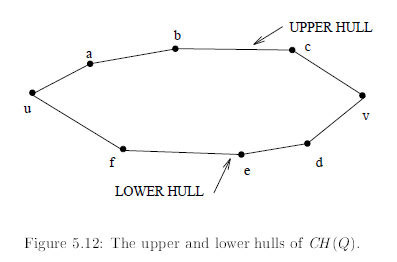
\includegraphics[width=\linewidth,center]{imgs/upper_lower_hull.png}

\end{frame}

\begin{frame}{Dealing with Merging}
Now, between each pair of hulls, we find a line that links the top of the hulls

This searching looks a lot like binary search.
		\begin{itemize}
			\item
				we start with both midpoints as ends to a line-segment.
			\item 
			    we test to see if any points in the hulls fall above the line generated
			\item
				if all the points fall below the line, then we have found a good linking.
			\item
			    otherwise, we need to eliminate some candidate edges
				
		\end{itemize}	

\end{frame}

\begin{frame}{Dealing with Merging}
	We can prune to the inside of the merge and below the tangent line.
		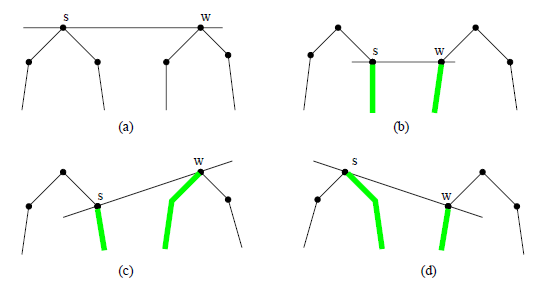
\includegraphics[width=\linewidth,center]{imgs/tangent_search.png}

\end{frame}

\begin{frame}{Dealing with Merging}
		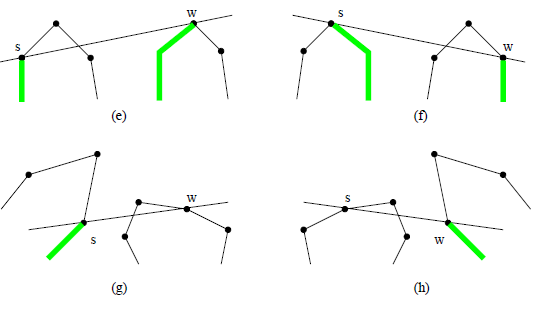
\includegraphics[width=\linewidth,center]{imgs/tangent_search_1.png}

\end{frame}


\end{frame}

\begin{frame}{Eliminating entire half-hulls}
	It is possible that an entire hull should be removed to prevent concavity
	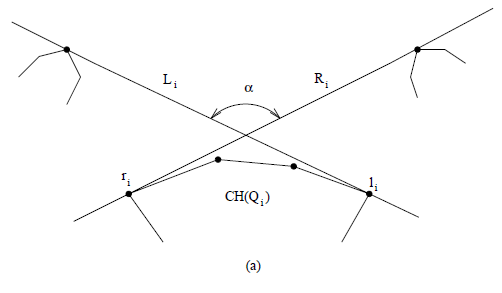
\includegraphics[width=\linewidth,center]{imgs/tangents.png}
\end{frame}

\begin{frame}{Eliminating entire half-hulls}
	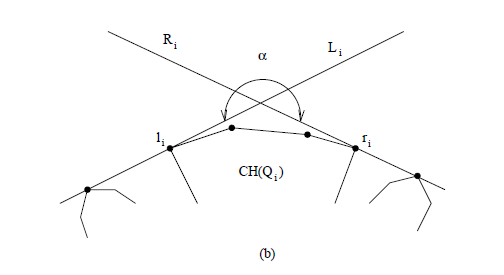
\includegraphics[width=\linewidth,center]{imgs/tangents_1.png}
\end{frame}

\begin{frame}{Complexity Summary}
	In the terminal recursion, it takes log(n) time to search for the pair of appropriate points on neighbouring hulls. All $n^\frac{1}{2^k}-1$ hull pairs can be merged in parallel.
	
	Each recursion uses $O(n^\frac{1}{2^k})$ processors to merge $O(n^\frac{1}{2^k})$ hulls each with $O(n^\frac{1}{2^{k+1}})$ points in $O(log(n^\frac{1}{2^k}))$ time.
	
	This results in a time complexity of $O(log(n^\frac{1}{2}))$ + $O(log(n^\frac{1}{4}))$ + $O(log(n^\frac{1}{8}))$ ... $O(log(n^\frac{1}{2^k}))$ which is equal to $O(log(n))$

\end{frame}




\section{CUDAHull}

\begin{frame}{Explain CUDAHull}
CUDAHhull is a O(log(n)) time and O(nlog(n)) work algorithm for find Convex hulls in 3d implemented on CUDA.

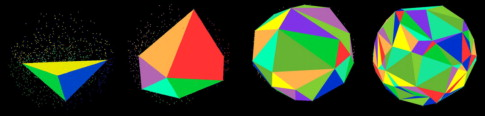
\includegraphics[scale=1]{imgs/CUDAhull_example.jpg} 

\end{frame}

\begin{frame}{Basic Algorithm}
\begin{itemize}
\item Build a big-tetrahedron in the middle of the space
\item Discard all points inside the tetrahedron. If there are no points, return
\item Recurse on each face of the Tetrahedron with points beyond the plane of that face
\item The face becomes a face of the next Tetrahedron
\end{itemize}
\end{frame}


\begin{frame}{How to built the first tetrahedron?}
\begin{itemize}
\item find the min-x and max-x points
\item find the point with maximum distance from that line
\item find the point with maximum distance from that plane
\end{itemize}
All these points are guaranteed to be part of the convex hull


For later tetrahedrons, you are provided a base triangle and form a tetrahedron with the available point furthest from that plane.

\end{frame}

\begin{frame}{Smoothing the Result}

	After the previous algorithm completes, we have the set of points in the convex hull however the polytopes described is not convex, it is "spiky".
	
	The a centralized fashion, examine the concavity of each of $O(n)$ edges and swap the vertices of concave cases. While this technically brings the time of the algorithm up to $O(n)$ time, in practice it accounts for less than 1\% of runtime.
	
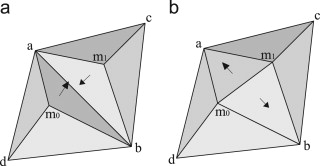
\includegraphics[scale=1]{imgs/CUDAHull-sampling.jpg} 


\end{frame}

\begin{frame}{Analysis}

CUDAHull uses O(n) processors to simultaneously search all recursive steps.
This creates a recursive tree of $log_4(n)$ depth and thus $O(nlog(n))$ work using O(n) processors in O(log(n)) time.

\end{frame}

% All of the following is optional and typically not needed. 
\appendix
\section<presentation>*{\appendixname}
\subsection<presentation>*{For Further Reading}

\end{document}


